% Provenance (never printed): see sources/outline_sources.md (Year 1:
% the Solar System, planetology). Kepler's laws, the moment of inertia and
% the Stefan--Boltzmann law are owned by the physics series and recalled
% here; the equilibrium temperature and the Bond albedo are re-founded from
% Book 2 grade 10. Curves computed in figdata/bachelor-1/planet_table.py;
% numbers of the exercises and problem in the Book 3 scratch calculator
% ch03.py.
\chapter{Planetologia comparada}\label{ch:b1:comparative-planetology}

Vênus e a Terra são quase gêmeas: Vênus tem \qty{95}{\percent} do raio da Terra e \qty{81}{\percent} da sua massa. No entanto a Terra tem oceanos, uma atmosfera de nitrogênio e oxigênio e placas em movimento, enquanto Vênus esconde sob as nuvens uma superfície a \qty{737}{K}, mais quente que qualquer forno de cozinha, esmagada por uma atmosfera de dióxido de carbono a \qty{92}{bar}. Marte, com a metade do tamanho da Terra, tem uma atmosfera fina e fria, vulcões gigantes e cânions, mas não tem placas em movimento. Mais longe, Júpiter e Saturno são sobretudo hidrogênio e hélio; Urano e Netuno, sobretudo os gelos de água, metano e amônia. Comparar os planetas é a única maneira de testar o que julgamos saber sobre a Terra: por que o seu interior é estratificado, por que o seu clima é ameno, por que só ela tem tectônica de placas. Este capítulo pesa e mede os planetas, lê os seus interiores a partir das densidades e da maneira como a massa se distribui, compara suas temperaturas e atmosferas, e termina com as luas e os pequenos corpos que guardam o registro da juventude do Sistema Solar.
% ledger: nasa:venus, earth:Rmean, earth:mass, nasa:uranus-structure

\begin{recall}
Os planetas giram em torno do Sol em elipses, e o quadrado do período de um satélite é proporcional ao cubo do seu semieixo maior (terceira lei de Kepler, no volume de física do primeiro ano, onde também se define o momento de inércia de um sólido; uma esfera homogênea tem $I = \tfrac25MR^2$). Um corpo negro irradia $\sigma T^4$ por unidade de área (no segundo ano). O Sistema Solar e os seus planetas rochosos e gigantes foram descritos no Livro 1 (6º ano); o albedo e a \omterm{def:b1:comparative-planetology:equilibrium-temperature}{temperatura de equilíbrio} de um planeta foram vistos no Livro 2 (10º ano), e o efeito estufa, no Livro 1 (9º ano).
\end{recall}

\begin{omfigure}
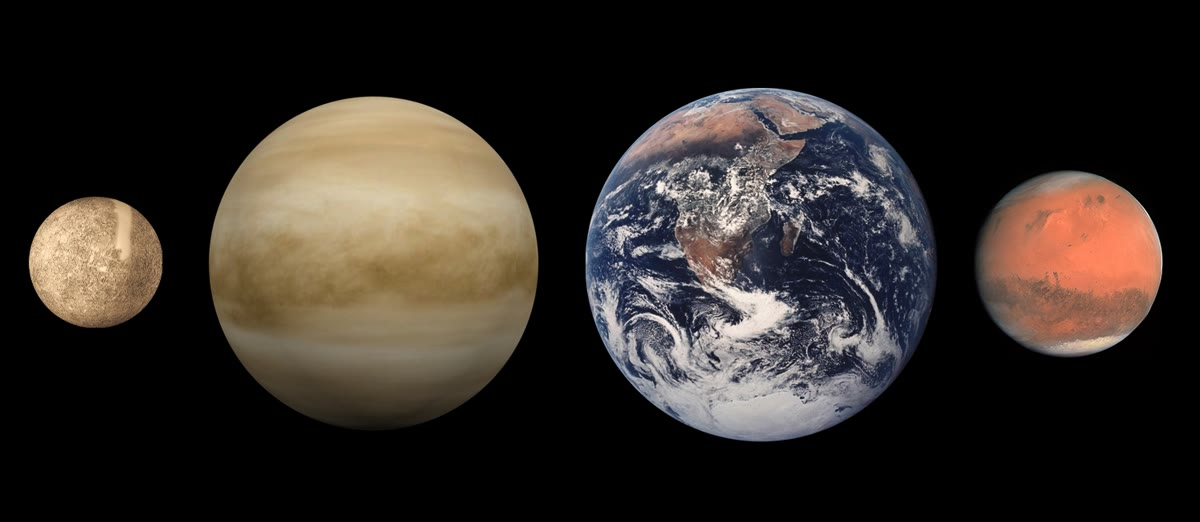
\includegraphics[width=0.85\linewidth]{images/book3/b1-terrestrial-planet-sizes.jpg}

{\small Os quatro planetas rochosos em escala, da esquerda para a direita Mercúrio, Vênus, a Terra e Marte (distâncias fora de escala; Vênus vista na luz visível, com a superfície escondida sob as nuvens). NASA, domínio público.}
% ledger: commons:terrestrial-sizes
\end{omfigure}

\section{Pesando e medindo os planetas}

O raio de um planeta é medido a partir do seu diâmetro angular e da sua distância, ou, para um planeta visitado por sondas, por altimetria de radar e de laser. Sua massa é mais difícil: ela só se manifesta pela atração gravitacional que o planeta exerce sobre outro corpo.

\begin{method}[A massa de um planeta a partir da órbita de um satélite]\label{met:b1:comparative-planetology:mass}
Para um satélite de massa desprezível, em uma órbita quase circular de raio (semieixo maior) $a$ e período sideral $T$ em torno de um planeta de massa $M$:
\begin{enumerate}
  \item converta $a$ para metros e $T$ para segundos;
  \item a terceira lei de Kepler dá $GM = 4\pi^2a^3/T^2$: esse produto é o que a órbita mede, e com precisão muito maior que a de $G$ em si;
  \item divida por $G = \qty{6.6743e-11}{m^3.kg^{-1}.s^{-2}}$ para obter $M$.
\end{enumerate}
Um planeta sem lua (Mercúrio, Vênus) é pesado do mesmo modo, a partir da órbita, ou do desvio, de uma sonda que passa por ele.
\end{method}

\begin{example}
Io, a maior lua interna de Júpiter, orbita a $a = \qty{421.8e3}{km}$
em \num{1.769138} dias, isto é, $T = \qty{152854}{s}$. Então
\[
  GM = \frac{4\pi^2\times(\qty{4.218e8}{m})^3}{(\qty{152854}{s})^2}
  = \qty{1.268e17}{m^3.s^{-2}}, \qquad
  M = \frac{\num{1.268e17}}{\num{6.6743e-11}} = \qty{1.900e27}{kg},
\]
o que concorda com a massa tabelada de Júpiter, \qty{1.898e27}{kg}, com \qty{0.1}{\percent}. A massa de Io, \num{4.7e-5} da de Júpiter, é desprezível; o pequeno excesso vem do abaulamento equatorial de Júpiter, que puxa uma lua próxima um pouco mais forte do que o faria uma esfera de mesma massa.
% ledger: nasa:io, nasa:jupiter, const:G
\end{example}

Com a massa e o raio vem a densidade média $\bar\rho =
3M/(4\pi R^3)$, a primeira pista do que é um planeta. As densidades dos planetas se dividem em dois grupos (veja a figura abaixo): Mercúrio, Vênus, a Terra e Marte situam-se entre cerca de \num{3900} e \qty{5500}{kg.m^{-3}}, mais densos do que qualquer rocha comum; os quatro planetas externos situam-se entre \num{690} e \qty{1640}{kg.m^{-3}}, perto da densidade da água, e Saturno até abaixo dela.
% ledger: planet:Mercury.density, planet:Mars.density, planet:Earth.density, planet:Saturn.density, planet:Neptune.density

\begin{omfigure}
\begin{tikzpicture}
\begin{axis}[omrecord, width=0.86\linewidth, height=6.2cm, xmode=log,
  xmin=800, xmax=150000, ymin=0, ymax=6300, xlabel={raio equatorial (km)},
  ylabel={densidade média (\unit{kg.m^{-3}})}, tick label style={font=\scriptsize},
  label style={font=\small}]
\addplot[only marks, mark=*, mark size=2.4pt, brown!70!black] table[x=R_km, y=density,
  restrict expr to domain={\thisrow{idx}}{0:2}] {figdata/out/bachelor-1-planet_table-bodies.dat};
\addplot[only marks, mark=*, mark size=2.4pt, brown!70!black] table[x=R_km, y=density,
  restrict expr to domain={\thisrow{idx}}{4:4}] {figdata/out/bachelor-1-planet_table-bodies.dat};
\addplot[only marks, mark=*, mark size=2.4pt, orange!85!black] table[x=R_km, y=density,
  restrict expr to domain={\thisrow{idx}}{5:6}] {figdata/out/bachelor-1-planet_table-bodies.dat};
\addplot[only marks, mark=*, mark size=2.4pt, omDef] table[x=R_km, y=density,
  restrict expr to domain={\thisrow{idx}}{7:8}] {figdata/out/bachelor-1-planet_table-bodies.dat};
\addplot[only marks, mark=o, mark size=2.4pt, black!60] table[x=R_km, y=density,
  restrict expr to domain={\thisrow{idx}}{3:3}] {figdata/out/bachelor-1-planet_table-bodies.dat};
\addplot[only marks, mark=o, mark size=2.4pt, black!60] table[x=R_km, y=density,
  restrict expr to domain={\thisrow{idx}}{9:9}] {figdata/out/bachelor-1-planet_table-bodies.dat};
\addplot[black!40, densely dashed] coordinates {(800,1000) (150000,1000)};
\begin{scope}[font=\scriptsize]
\node[left] at (axis cs:2439.5,5429) {Mercúrio};
\node[below left] at (axis cs:6052,5243) {Vênus};
\node[above] at (axis cs:6378,5514) {Terra};
\node[left] at (axis cs:3396,3934) {Marte};
\node[left] at (axis cs:1737.5,3340) {Lua};
\node[right] at (axis cs:1188,1850) {Plutão};
\node[above] at (axis cs:71492,1326) {Júpiter};
\node[left] at (axis cs:60268,687) {Saturno};
\node[right] at (axis cs:25559,1270) {Urano};
\node[above] at (axis cs:24764,1638) {Netuno};
\node[above left, black!60] at (axis cs:150000,1000) {água};
\end{scope}
\end{axis}
\end{tikzpicture}

{\small Densidade média em função do raio (escala logarítmica) dos oito planetas (cheios: rochosos, \omterm{def:b1:comparative-planetology:planet-types}{gigantes gasosos} e \omterm{def:b1:comparative-planetology:planet-types}{gigantes de gelo}), da Lua e de Plutão (círculos vazios). Dados da ficha planetária da NASA.}
% ledger: planet:Mercury.diameter, planet:Venus.diameter, planet:Earth.diameter, planet:Moon.diameter, planet:Mars.diameter, planet:Jupiter.diameter, planet:Saturn.diameter, planet:Uranus.diameter, planet:Neptune.diameter, planet:Pluto.diameter, planet:Mercury.density, planet:Venus.density, planet:Earth.density, planet:Moon.density, planet:Mars.density, planet:Jupiter.density, planet:Saturn.density, planet:Uranus.density, planet:Neptune.density, planet:Pluto.density
\end{omfigure}

A densidade média, sozinha, não consegue dizer se um planeta é feito de um só material denso ou se tem um centro muito denso e um envelope mais leve. Um segundo número consegue: como a massa se distribui entre o centro e a superfície.

\begin{definition}[Fator de momento de inércia]\label{def:b1:comparative-planetology:moi}
O \emph{fator de momento de inércia}\index{fator de momento de inércia} de um planeta é o número
\[
  C = \frac{I}{MR^2} ,
\]
onde $I$ é o seu momento de inércia em torno do eixo de rotação, $M$ a sua massa e $R$ o seu raio médio. Uma esfera homogênea tem $C = \tfrac25 = 0.4$; um planeta cuja densidade cresce em direção ao centro tem $C < 0.4$, tanto menor quanto mais a massa estiver concentrada.
\end{definition}

O momento de inércia é medido a partir da lenta precessão do eixo de rotação sob a atração do Sol, junto com o achatamento do campo gravitacional do planeta. Os valores são reveladores: a Lua, com $C = 0.394$, é quase homogênea; Marte, com $0.366$, e a Terra, com $0.3308$, são claramente estratificados; Júpiter, com $0.254$, e Saturno, com $0.210$, têm a maior parte da massa concentrada em direção ao centro.
% ledger: nasa:moon, nasa:mars, earth:MoI, nasa:jupiter, nasa:saturn

\section{Do que são feitos os planetas}

\begin{definition}[Planetas terrestres e gigantes]\label{def:b1:comparative-planetology:planet-types}
Um \emph{planeta terrestre}\index{planeta terrestre} é um planeta feito sobretudo de rocha silicatada e ferro, com superfície sólida: Mercúrio, Vênus, a Terra e Marte. Um \emph{planeta gigante}\index{planeta gigante} é um planeta muitas vezes mais massivo que a Terra, feito sobretudo de elementos leves e seus compostos, e sem superfície sólida. Um \emph{gigante gasoso}\index{gigante gasoso} é um planeta gigante feito sobretudo de hidrogênio e hélio: Júpiter e Saturno. Um \emph{gigante de gelo}\index{gigante de gelo} é um planeta gigante feito sobretudo dos compostos que os astrônomos chamam de gelos --- água, metano e amônia --- sob um envelope de hidrogênio e hélio: Urano e Netuno.
\end{definition}

As atmosferas que as sondas e os telescópios medem confirmam a divisão. A de Júpiter é de \qty{89.8}{\percent} de hidrogênio e \qty{10.2}{\percent} de hélio em volume, a de Saturno, \qty{96.3}{\percent} e \qty{3.25}{\percent}; no caso de Urano, pelo menos \qty{80}{\percent} da massa é um fluido denso e quente de água, metano e amônia sobre um pequeno núcleo rochoso. A densidade média de um \omterm{def:b1:comparative-planetology:planet-types}{gigante gasoso} permanece baixa, embora o seu centro seja fortemente comprimido, porque o hidrogênio é o elemento mais leve; um \omterm{def:b1:comparative-planetology:planet-types}{gigante de gelo} é mais denso que Saturno porque os seus gelos são mais pesados que o hidrogênio.
% ledger: nasa:jupiter, nasa:saturn, nasa:uranus-structure

Os \omterm{def:b1:comparative-planetology:planet-types}{planetas terrestres} são estratificados como a Terra: um núcleo rico em ferro sob um manto silicatado e uma crosta fina. O modelo mais simples que usa os dois números medidos, a densidade média e o \omterm{def:b1:comparative-planetology:moi}{fator de momento de inércia}, tem duas camadas.

\begin{proposition}[O planeta de duas camadas]\label{prop:b1:comparative-planetology:two-layer}
Considere um planeta de raio $R$ como um núcleo de raio $xR$ e densidade uniforme $\rho_c$ dentro de um manto de densidade uniforme $\rho_m$. Sua densidade média e seu \omterm{def:b1:comparative-planetology:moi}{fator de momento de inércia} são
\[
  \bar\rho = \rho_m + (\rho_c - \rho_m)\,x^3 , \qquad
  C = \frac25\,\frac{\rho_m + (\rho_c - \rho_m)\,x^5}{\bar\rho} .
\]
Dados $\bar\rho$, $C$ e uma densidade presumida para o manto, $\rho_m$, o raio relativo do núcleo segue:
\[
  x^2 = \frac{\tfrac52C\bar\rho - \rho_m}{\bar\rho - \rho_m} ,
  \qquad \rho_c = \rho_m + \frac{\bar\rho - \rho_m}{x^3} .
\]
\end{proposition}

\begin{proof}
O planeta é uma esfera homogênea de densidade $\rho_m$ e raio $R$, mais uma esfera de raio $xR$ com o excesso de densidade $\rho_c - \rho_m$. As massas se somam: $M = \tfrac43\pi R^3[\rho_m + (\rho_c - \rho_m)x^3]$, e dividindo pelo volume obtém-se $\bar\rho$. Os momentos de inércia em torno do mesmo eixo também se somam; uma esfera homogênea de densidade $\rho$ e raio $r$ tem
$I = \tfrac25\cdot\tfrac43\pi\rho r^3\cdot r^2 = \tfrac{8\pi}{15}\rho r^5$,
logo $I = \tfrac{8\pi}{15}R^5[\rho_m + (\rho_c - \rho_m)x^5]$. Dividindo por $MR^2 = \tfrac43\pi\bar\rho R^5$ obtém-se $C$. Por fim, as duas equações ficam $(\rho_c - \rho_m)x^3 = \bar\rho - \rho_m$ e $(\rho_c - \rho_m)x^5 =
\tfrac52C\bar\rho - \rho_m$; dividindo a segunda pela primeira obtém-se $x^2$, e a primeira dá $\rho_c$.
\end{proof}

O modelo tem três incógnitas e dois dados, de modo que uma delas, a densidade do manto, deve ser presumida a partir do que rochas de composição adequada pesam sob pressão. A resposta é sensível a essa escolha quando $C$ está perto de $0.4$, porque $\tfrac52C\bar\rho - \rho_m$ é então uma pequena diferença de números grandes (\cref{exo:b1:comparative-planetology:10} e o problema). O modelo também ignora a compressão do manto pelo próprio peso, que, num planeta do tamanho da Terra, eleva a densidade do manto profundo bem acima da das rochas da superfície; para a Terra, a sismologia faz muito melhor (\cref{ch:b1:layered-earth}). Sismômetros colocados em Marte fizeram agora o mesmo para esse planeta: onde a tabela planetária dá um raio de núcleo de \qty{1830}{km}, os resultados recentes indicam apenas \qty{1650}{km} a \qty{1675}{km}.
% ledger: nasa:mars-core

\begin{omfigure}
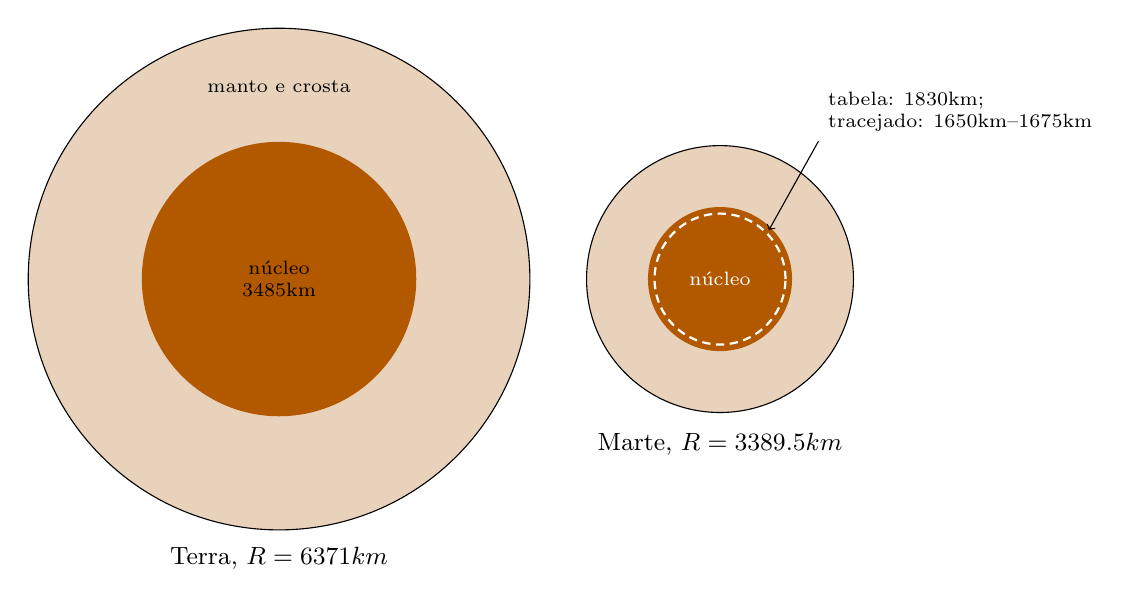
\begin{tikzpicture}[font=\scriptsize]
% scale: 0.5 cm per 1000 km
\fill[brown!35] (0,0) circle (3.1855cm);
\fill[orange!70!black] (0,0) circle (1.7425cm);
\draw (0,0) circle (3.1855cm);
\node[align=center] at (0,0) {núcleo\\ \qty{3485}{km}};
\node[align=center] at (0,2.45) {manto e crosta};
\node at (0,-3.55) {\small Terra, $R = \qty{6371}{km}$};
\begin{scope}[xshift=5.6cm]
\fill[brown!35] (0,0) circle (1.6948cm);
\fill[orange!70!black] (0,0) circle (0.915cm);
\draw[white, densely dashed, thick] (0,0) circle (0.8313cm);
\draw (0,0) circle (1.6948cm);
\node[align=center, white] at (0,0) {núcleo};
\node at (0,-2.1) {\small Marte, $R = \qty{3389.5}{km}$};
\draw[->] (1.25,1.75) node[above right, align=left] {tabela: \qty{1830}{km};\\ tracejado: \qty{1650}{km}--\qty{1675}{km}} -- (0.62,0.62);
\end{scope}
\end{tikzpicture}

{\small A Terra e Marte em escala, com os seus núcleos. Para Marte, a borda cheia é o raio do núcleo da tabela planetária, e o círculo tracejado é o raio menor indicado pelos resultados sísmicos recentes. Os dois núcleos são ricos em ferro; o da Terra tem uma parte interna sólida, que não está desenhada.}
% ledger: earth:Rmean, earth:Rcore, nasa:mars, nasa:mars-core
\end{omfigure}

\section{Atmosferas e superfícies}

A temperatura de um planeta é fixada, em primeiro lugar, pela luz solar que ele absorve. A irradiância $S$ a uma distância $d$ do Sol cai como $1/d^2$ (\cref{prop:b1:observing-the-sky:inverse-square}): \qty{1361}{W.m^{-2}} na Terra, \qty{2601}{W.m^{-2}} em Vênus, \qty{586}{W.m^{-2}} em Marte, \qty{50}{W.m^{-2}} em Júpiter. Parte dela é refletida de volta, diretamente.
% ledger: earth:TSI, nasa:venus, nasa:mars, nasa:jupiter

\begin{definition}[Albedo de Bond]\label{def:b1:comparative-planetology:albedo}
O \emph{albedo de Bond}\index{albedo de Bond} $A$ de um planeta é a fração da potência total da luz solar que incide sobre ele e que ele reflete e espalha de volta ao espaço, em todos os comprimentos de onda e em todas as direções.
\end{definition}

Neve fresca e nuvens brilhantes refletem muito; rocha escura e mar aberto, pouco. Vênus, envolto em nuvens brilhantes, tem $A = 0.77$; a Terra, $0.294$; Marte, $0.250$; a Lua, rocha cinzenta escura, $0.11$.
% ledger: nasa:venus, earth:albedo, nasa:mars, nasa:moon

\begin{definition}[Temperatura de equilíbrio]\label{def:b1:comparative-planetology:equilibrium-temperature}
A \emph{temperatura de equilíbrio}\index{temperatura de equilíbrio} $T_\mathrm{eq}$ de um planeta é a temperatura uniforme à qual um corpo negro do tamanho do planeta irradiaria para o espaço exatamente a potência que o planeta absorve do Sol.
\end{definition}

\begin{proposition}[Temperatura de equilíbrio]\label{prop:b1:comparative-planetology:teq}
Um planeta de \omterm{def:b1:comparative-planetology:albedo}{albedo de Bond} $A$ que recebe a irradiância $S$ tem
\[
  T_\mathrm{eq} = \left(\frac{S(1 - A)}{4\sigma}\right)^{1/4},
  \qquad \sigma = \qty{5.6704e-8}{W.m^{-2}.K^{-4}} .
\]
\end{proposition}

\begin{proof}
O planeta intercepta a luz solar que incide sobre a sua seção transversal, um disco de área $\pi R^2$, e absorve a fração $1 - A$: absorve $S(1 - A)\pi
R^2$. Um corpo negro (lei de Stefan--Boltzmann, recordada do volume de física do segundo ano) à temperatura uniforme $T$ irradia $\sigma T^4$ de cada metro quadrado de toda a sua superfície, $4\pi R^2$. Igualando as duas potências,
$4\pi R^2\sigma T^4 = S(1 - A)\pi R^2$, e o fator 4 é a razão entre a área da esfera e a sua seção transversal.
\end{proof}

Com os valores acima, $T_\mathrm{eq}$ é \qty{255}{K} para a Terra, \qty{227}{K} para Vênus, \qty{210}{K} para Marte e \qty{270}{K} para a Lua. Vênus, embora mais próxima do Sol, sai mais fria que a Terra: suas nuvens refletem três quartos da luz solar. A figura abaixo põe esses valores ao lado das temperaturas médias da superfície medidas. As diferenças são o efeito estufa, que os parágrafos seguintes e os capítulos sobre o clima (\cref{ch:b1:radiation-heat-transport}) tornam quantitativo: cerca de \qty{33}{K} para a Terra, cerca de \qty{510}{K} para Vênus, apenas cerca de \qty{4}{K} para Marte.
% ledger: const:sigma, earth:Tsurf, nasa:venus, nasa:mars, planet:Moon.Tmean

\begin{omfigure}
\begin{tikzpicture}
\begin{axis}[ybar, bar width=12pt, width=0.72\linewidth, height=5.8cm,
  ymin=0, ymax=820, xmin=-0.6, xmax=3.6, xtick={0,1,2,3},
  xticklabels={Lua, Marte, Terra, Vênus}, ylabel={temperatura (K)},
  tick label style={font=\scriptsize}, label style={font=\small},
  ymajorgrids, grid style={black!12}, axis lines*=left,
  legend style={font=\scriptsize, at={(0.03,0.97)}, anchor=north west, draw=none},
  nodes near coords, nodes near coords style={font=\tiny},
  every node near coord/.append style={/pgf/number format/fixed, /pgf/number format/precision=0}]
\addplot[fill=omDef!55, draw=omDef] table[x=idx, y=Teq] {figdata/out/bachelor-1-planet_table-temps.dat};
\addplot[fill=omThm!60, draw=omThm] table[x=idx, y=Tsurf] {figdata/out/bachelor-1-planet_table-temps.dat};
\legend{temperatura de equilíbrio, temperatura média da superfície}
\end{axis}
\end{tikzpicture}

{\small \omterm{def:b1:comparative-planetology:equilibrium-temperature}{Temperatura de equilíbrio} (calculada a partir da irradiância e do \omterm{def:b1:comparative-planetology:albedo}{albedo de Bond}) e temperatura média medida na superfície de quatro corpos. A atmosfera aquece a Terra e, sobretudo, Vênus; a atmosfera fina de Marte pouco faz; a Lua, sem ar, é em média mais fria que a sua \omterm{def:b1:comparative-planetology:equilibrium-temperature}{temperatura de equilíbrio}.}
% ledger: nasa:moon, nasa:mars, earth:TSI, earth:albedo, earth:Tsurf, nasa:venus, planet:Moon.Tmean, const:sigma
\end{omfigure}

A temperatura média da Lua, de cerca de \qty{253}{K}, fica abaixo da sua \omterm{def:b1:comparative-planetology:equilibrium-temperature}{temperatura de equilíbrio}. Isso não é um paradoxo: sem atmosfera nem oceano para transportar calor, o lado iluminado é muito quente e o lado noturno muito frio, e, como a emissão cresce com $T^4$, um corpo de temperaturas desiguais irradia a potência absorvida com uma temperatura média menor do que um corpo uniforme (\cref{exo:b1:comparative-planetology:11}).

Uma atmosfera faz duas coisas: deixa passar a maior parte da luz solar e absorve parte do infravermelho que o solo emite, reirradiando uma parte dele para baixo. Quanto ela aquece a superfície depende de quanto gás absorvente há acima de cada metro quadrado. A pressão na superfície mede exatamente isso: $p = mg$ para uma coluna de massa $m$ por metro quadrado. A atmosfera de Vênus, a \qty{92}{bar}, é \qty{96.5}{\percent} de dióxido de carbono; a de Marte, com apenas \qty{6.36}{mbar} em média, é também \qty{95.1}{\percent} de dióxido de carbono, mas tem cerca de sessenta vezes menos gás acima de cada metro quadrado do que a da Terra, e muito pouco vapor de água. Os dois planetas têm atmosferas de dióxido de carbono; só um deles tem uma atmosfera espessa.
% ledger: nasa:venus, nasa:mars, earth:psurf

\begin{omfigure}
\begin{minipage}{0.4\linewidth}
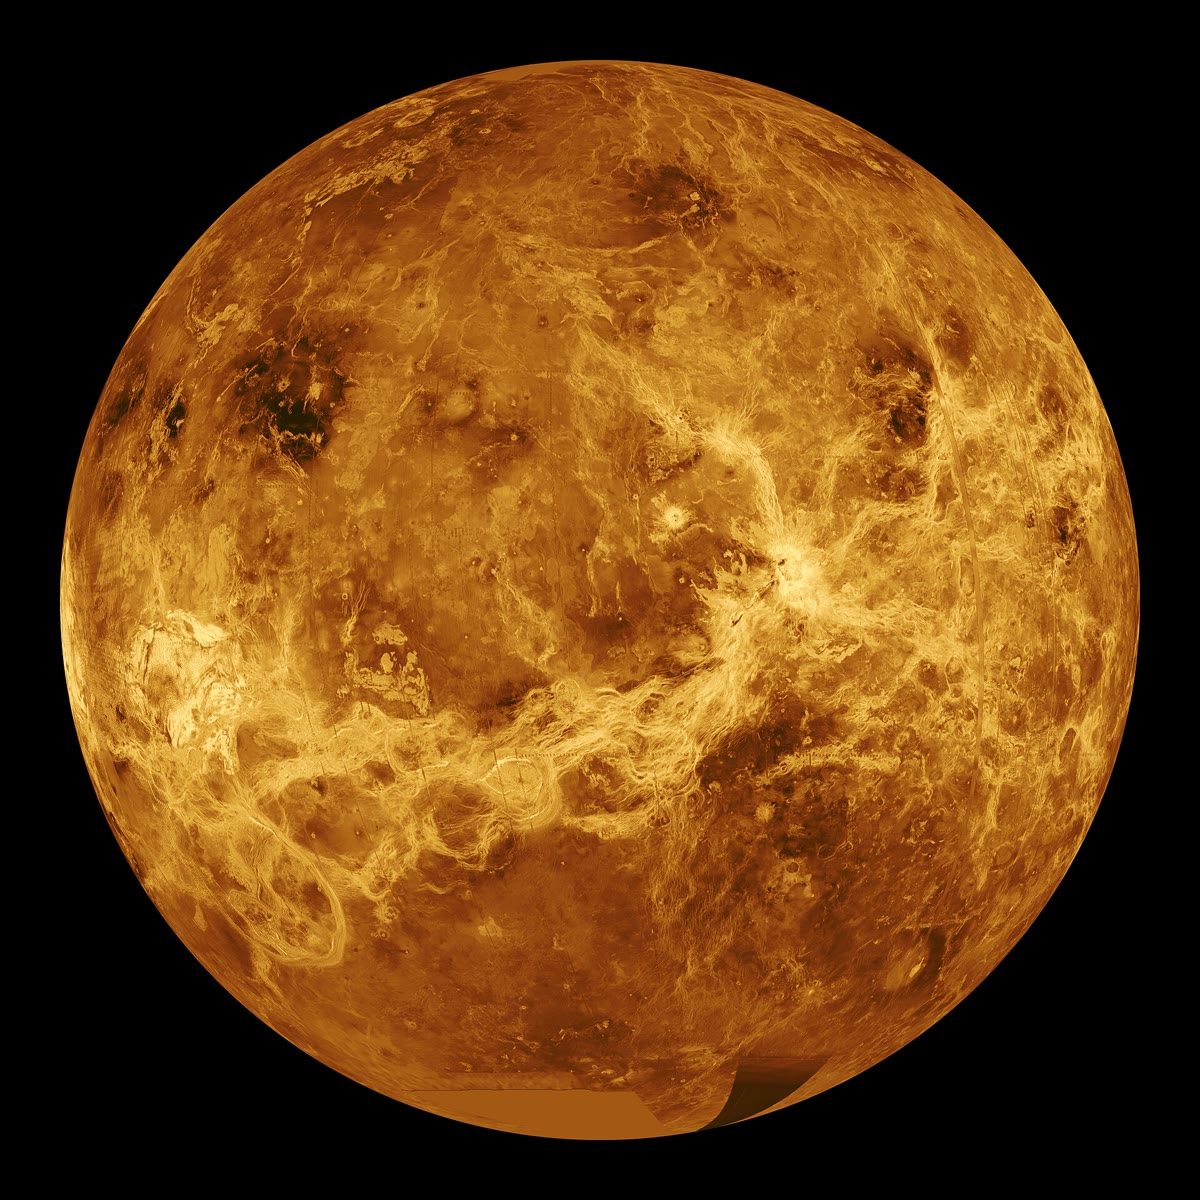
\includegraphics[width=\linewidth]{images/book3/b1-venus-radar-globe.jpg}
\end{minipage}\hspace{0.06\linewidth}
\begin{minipage}{0.4\linewidth}
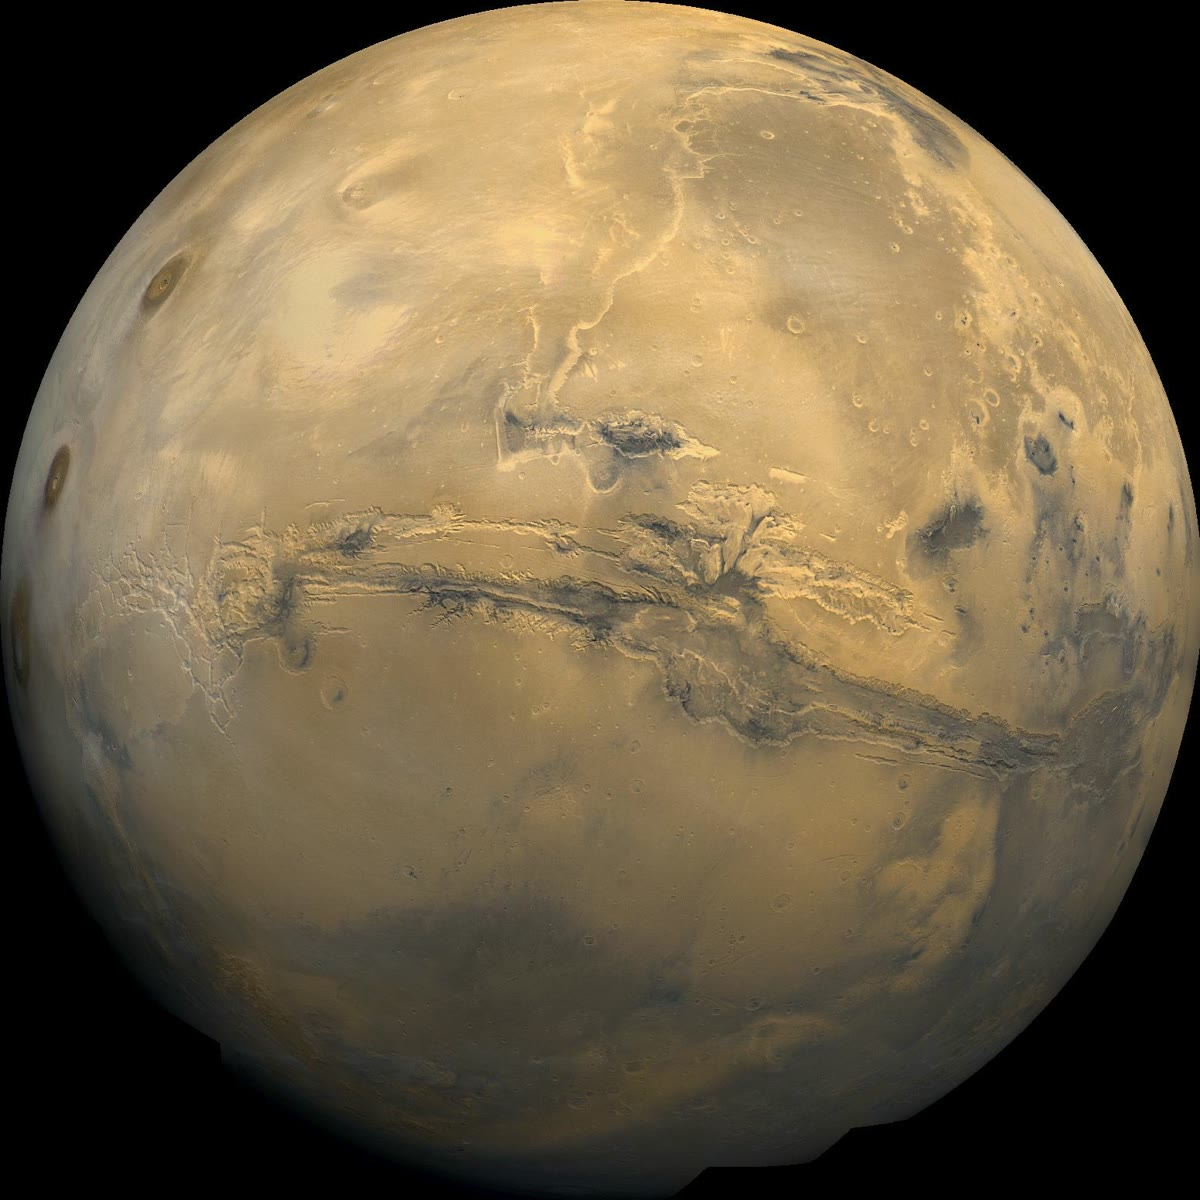
\includegraphics[width=\linewidth]{images/book3/b1-mars-valles-marineris.jpg}
\end{minipage}

{\small À esquerda: a superfície de Vênus vista através das nuvens pelo radar da sonda Magellan, mapeada sobre um globo simulado por computador (as cores são simuladas). À direita: Marte vista pela sonda Viking 1, um mosaico centrado no sistema de cânions de Valles Marineris. NASA/JPL e NASA/USGS, domínio público.}
% ledger: commons:venus-globe, commons:mars-valles
\end{omfigure}

As superfícies guardam o registro do que as moldou. Crateras de impacto se acumulam em qualquer superfície exposta ao espaço; uma superfície muito craterada, como a maior parte da Lua ou de Mercúrio, é antiga, e uma superfície com poucas crateras foi renovada: por fluxos de lava, pela erosão ou pelas placas que levam o assoalho oceânico da Terra de volta ao manto. Planícies vulcânicas e vulcões são encontrados em todos os \omterm{def:b1:comparative-planetology:planet-types}{planetas terrestres}. Falhas, riftes e cinturões dobrados mostram que as litosferas de Vênus e de Marte foram deformadas; mas, de todos os planetas, só a Terra mostra hoje uma litosfera partida em placas que se movem como blocos rígidos, com dorsais onde se formam e fossas onde afundam. Por que só a Terra tem tectônica de placas ainda é discutido; a presença de água, que enfraquece as rochas, é uma das razões propostas.

\section{Luas e pequenos corpos}

A Lua, com um quarto do diâmetro da Terra, é grande para um satélite. Sua densidade, \qty{3340}{kg.m^{-3}}, próxima à das rochas do manto terrestre, e seu \omterm{def:b1:comparative-planetology:moi}{fator de momento de inércia}, próximo de $0.4$, mostram que ela tem no máximo um pequeno núcleo de ferro. Os \omterm{def:b1:comparative-planetology:planet-types}{planetas gigantes} têm sistemas de luas que são mundos em si mesmos (veja as fotografias abaixo). Io, a mais interna das quatro grandes luas de Júpiter, é o mundo mais ativo vulcanicamente do Sistema Solar, com centenas de vulcões, aquecida pelas marés que Júpiter nela provoca; o vulcanismo a renova mais depressa do que os impactos conseguem marcá-la com grandes crateras. Europa, de densidade \qty{3010}{kg.m^{-3}}, é rocha sob uma crosta de gelo, e há forte indício de um oceano salgado sob essa crosta. Ganimedes e Calisto, de densidades \num{1940} e \qty{1830}{kg.m^{-3}}, são feitas de rocha e gelo em quantidades comparáveis.
Titã, a maior lua de Saturno, é a única lua com uma atmosfera densa, sobretudo de nitrogênio com um pouco de metano, e o único mundo, além da Terra, com rios, lagos e mares na superfície --- de metano e etano líquidos; ele também provavelmente esconde um oceano de água.
% ledger: planet:Moon.diameter, planet:Earth.diameter, planet:Moon.density, nasa:moon, nasa:io-facts, nasa:europa, nasa:europa-facts, nasa:ganymede, nasa:titan-facts

\begin{omfigure}
\begin{minipage}{0.4\linewidth}
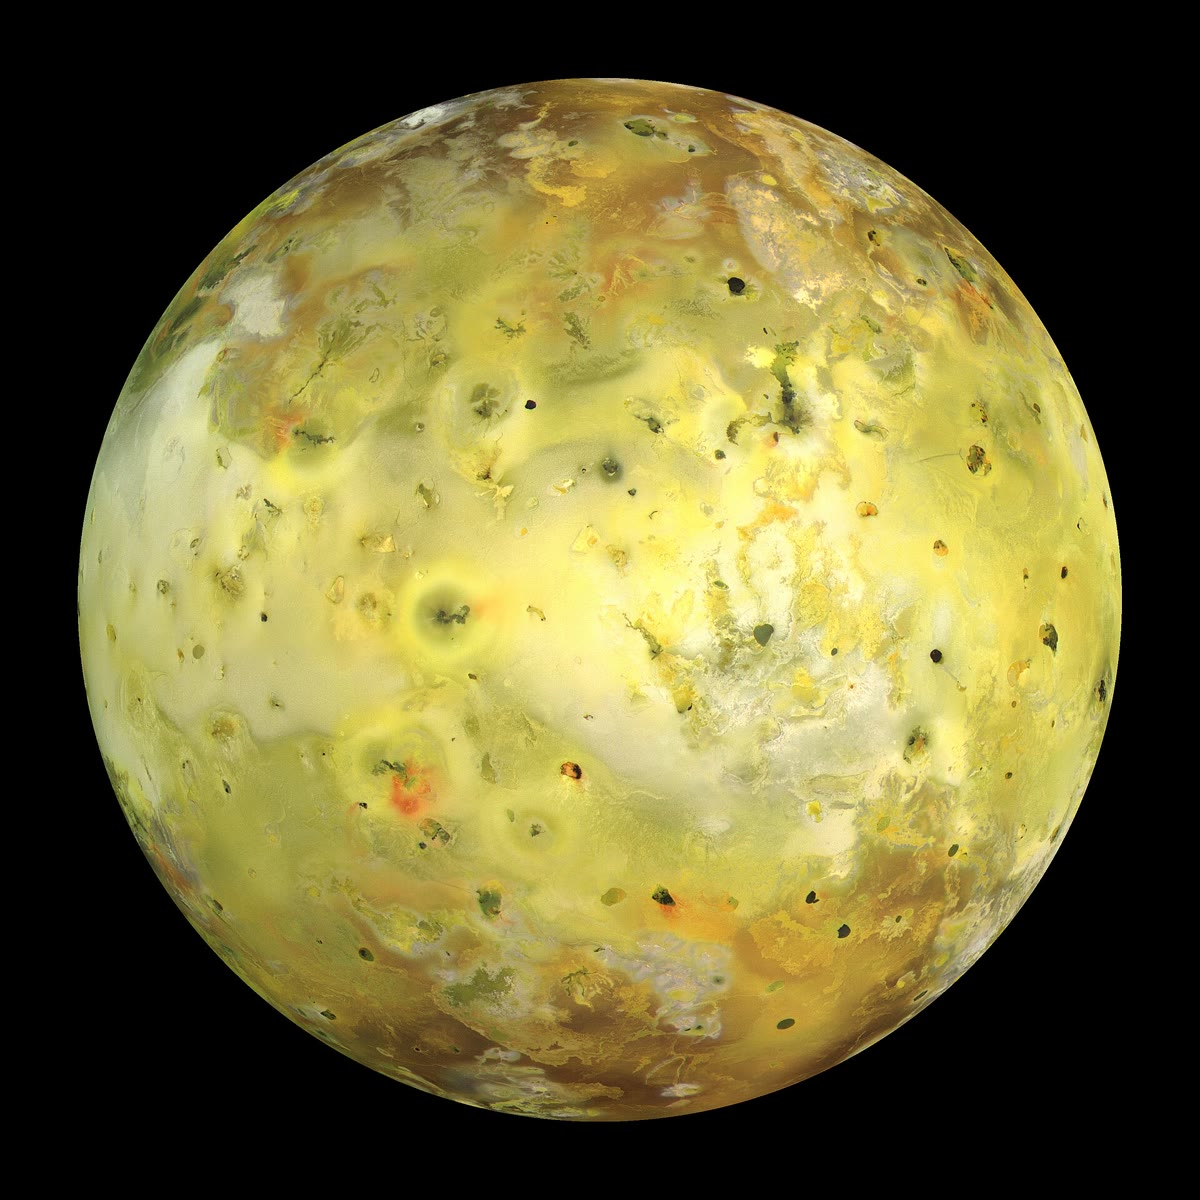
\includegraphics[width=\linewidth]{images/book3/b1-io.jpg}
\end{minipage}\hspace{0.06\linewidth}
\begin{minipage}{0.4\linewidth}
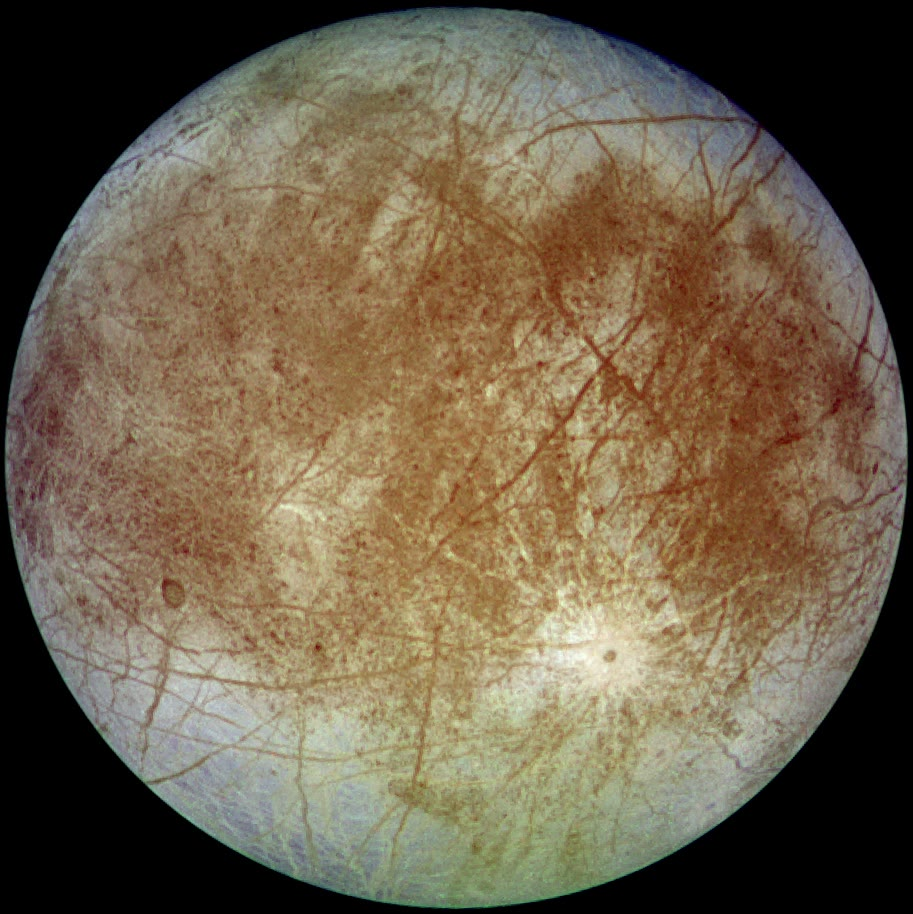
\includegraphics[width=\linewidth]{images/book3/b1-europa.jpg}
\end{minipage}

{\small Duas das grandes luas de Júpiter vistas pela sonda Galileo. À esquerda, Io, com a superfície pontilhada de centros vulcânicos e colorida por compostos de enxofre e lavas. À direita, Europa em cor natural aproximada; as longas linhas escuras são fraturas em sua crosta de gelo. NASA/JPL/University of Arizona e NASA/JPL/DLR, domínio público.}
% ledger: commons:io, commons:europa, nasa:io-facts, nasa:europa
\end{omfigure}

\begin{definition}[Asteroide, cometa, objeto transnetuniano]\label{def:b1:comparative-planetology:small-bodies}
Um \emph{asteroide}\index{asteroide} é um pequeno corpo rochoso ou metálico que orbita o Sol, pequeno demais para ser um planeta e sem o envelope de gás e poeira de um cometa; a maioria orbita entre Marte e Júpiter. Um \emph{cometa}\index{cometa} é um pequeno corpo de gelo e poeira que, quando sua órbita o aproxima do Sol, libera gás e poeira que formam um envoltório luminoso em torno dele e caudas apontando para longe do Sol. Um \emph{objeto transnetuniano}\index{objeto transnetuniano} é um corpo do Sistema Solar cuja órbita fica, em média, além da de Netuno.
\end{definition}

Os \omterm{def:b1:comparative-planetology:small-bodies}{objetos transnetunianos} do Cinturão de Kuiper, uma zona em forma de disco além de Netuno, são corpos de gelo e rocha restos da formação dos planetas; Plutão, classificado como planeta anão desde 2006, é um deles. Os \omterm{def:b1:comparative-planetology:small-bodies}{asteroides} são os destroços de uma região onde nenhum planeta se formou. Fragmentos de \omterm{def:b1:comparative-planetology:small-bodies}{asteroides}, e alguns da Lua e de Marte, caem sobre a Terra como meteoritos. São as únicas amostras de outros mundos em nossas mãos, além das trazidas por sondas, e alguns deles mudaram pouco desde a formação do Sistema Solar; suas classes, e o que dizem sobre a composição da Terra e a idade do Sistema Solar, são o assunto do Livro 4.
% ledger: nasa:pluto-facts

\section{Exercícios}

\begin{exercise}[$\star$]\label{exo:b1:comparative-planetology:1}
Júpiter tem massa de \qty{1898.13e24}{kg} e raio médio de \qty{69911}{km}. Calcule sua densidade média e compare-a com a da água, \qty{1000}{kg.m^{-3}}.
\end{exercise}

\begin{exercise}[$\star$]\label{exo:b1:comparative-planetology:2}
Usando a figura das densidades e dos raios, classifique Mercúrio, Saturno, Urano e Vênus como \omterm{def:b1:comparative-planetology:planet-types}{planetas terrestres}, \omterm{def:b1:comparative-planetology:planet-types}{gigantes gasosos} ou \omterm{def:b1:comparative-planetology:planet-types}{gigantes de gelo}, e justifique cada escolha pelo seu raio e pela sua densidade.
\end{exercise}

\begin{exercise}[$\star$]\label{exo:b1:comparative-planetology:3}
Vênus recebe \qty{2601.3}{W.m^{-2}} e tem \omterm{def:b1:comparative-planetology:albedo}{albedo de Bond} de 0.77. Calcule sua \omterm{def:b1:comparative-planetology:equilibrium-temperature}{temperatura de equilíbrio}. Por que ela é mais baixa que a da Terra, embora Vênus esteja mais perto do Sol?
\end{exercise}

\begin{exercise}[$\star$]\label{exo:b1:comparative-planetology:4}
Ordene a Lua ($C = 0.394$), Marte (0.366), a Terra (0.3308), Júpiter (0.254) e Saturno (0.210) do mais homogêneo ao mais concentrado no centro. Qual seria $C$ para um planeta cuja massa inteira estivesse concentrada em um ponto no seu centro?
\end{exercise}

\begin{exercise}[$\star\star$]\label{exo:b1:comparative-planetology:5}
Titã orbita Saturno a $a = \qty{1221.87e3}{km}$ em \num{15.945421} dias. Calcule a massa de Saturno e compare-a com o valor tabelado de \qty{568.32e24}{kg}.
\end{exercise}

\begin{exercise}[$\star\star$]\label{exo:b1:comparative-planetology:6}
A Terra recebe \qty{1361}{W.m^{-2}} a \qty{149.6e6}{km} do Sol. Calcule a irradiância em Marte (\qty{228.0e6}{km}) e em Júpiter (\qty{778.5e6}{km}), e compare-as com os valores tabelados de \qty{586.2}{W.m^{-2}} e \qty{50.26}{W.m^{-2}}.
\end{exercise}

\begin{exercise}[$\star\star$]\label{exo:b1:comparative-planetology:7}
Mostre que, para um dado albedo, $T_\mathrm{eq}$ varia como $d^{-1/2}$. Calcule $T_\mathrm{eq}$ para Júpiter ($S = \qty{50.26}{W.m^{-2}}$, $A = 0.343$). Se fosse constatado que Júpiter irradia mais potência do que absorve do Sol, o que isso implicaria sobre o seu interior?
\end{exercise}

\begin{exercise}[$\star\star$]\label{exo:b1:comparative-planetology:8}
Calcule o aquecimento por efeito estufa, $T_\mathrm{surf} - T_\mathrm{eq}$, de Vênus (\qty{737}{K}), da Terra (\qty{288}{K}, $A = 0.294$) e de Marte (\qty{214}{K}). Exprima cada um como fração de $T_\mathrm{eq}$.
\end{exercise}

\begin{exercise}[$\star\star$]\label{exo:b1:comparative-planetology:9}
Para uma esfera homogênea, mostre que $C = 0.4$ integrando os momentos de inércia de cascas esféricas finas (uma casca de raio $r$ e massa $\mathrm dm$ tem $\mathrm dI = \tfrac23 r^2\,\mathrm dm$). Que valor tem uma casca oca de raio $R$?
\end{exercise}

\begin{exercise}[$\star\star\star$]\label{exo:b1:comparative-planetology:10}
Mercúrio tem $\bar\rho = \qty{5429}{kg.m^{-3}}$, $C = 0.35$ e raio de \qty{2439.7}{km}. Com uma densidade de manto de \qty{3300}{kg.m^{-3}}, use o modelo de duas camadas para encontrar o raio do seu núcleo, a densidade do núcleo e a fração de sua massa no núcleo. O que há de notável em Mercúrio?
\end{exercise}

\begin{exercise}[$\star\star\star$]\label{exo:b1:comparative-planetology:11}
Modele um corpo sem ar cujo hemisfério diurno está à temperatura uniforme $T_1$ e o noturno a $T_2$, irradiando juntos a potência absorvida. (a) Mostre que, se $T_1^4 + T_2^4 = 2T_\mathrm{eq}^4$, a temperatura média $(T_1 + T_2)/2$ é no máximo $T_\mathrm{eq}$, com igualdade apenas quando $T_1 = T_2$. (b) Para a Lua, $T_\mathrm{eq} = \qty{270}{K}$; tome $T_2 = \qty{100}{K}$. Calcule $T_1$ e a temperatura média.
\end{exercise}

\begin{exercise}[$\star\star\star$]\label{exo:b1:comparative-planetology:12}
Vênus tem raio de \qty{6051.8}{km}, gravidade na superfície de \qty{8.9}{m.s^{-2}} e pressão superficial de \qty{92}{bar}. Calcule a massa de sua atmosfera, compare-a com a da atmosfera terrestre, \qty{5.1e18}{kg}, e com a massa de Vênus, \qty{4.8673e24}{kg}. O que a comparação sugere sobre onde está guardado o dióxido de carbono da Terra?
% ledger: earth:Matm, planet:Venus.gravity, nasa:venus
\end{exercise}

\section{Problema: pesando e sondando Marte}

\begin{problem}[{Problema de fim de semana --- a massa de Marte a partir da sua lua, da sua densidade e temperatura, e o tamanho do seu núcleo}]
\label{pb:b1:comparative-planetology:1}
% ledger: nasa:phobos, nasa:mars, nasa:mars-core, const:G, const:sigma, earth:psurf, earth:gmean, planet:Mars.Prot, planet:Earth.density
% numbers computed in the scratch calculator calc/ch03.py from the rounded data
Fobos, a maior lua de Marte, orbita a uma distância média de
\qty{9378}{km} do centro de Marte em \num{0.31891} dias. Marte tem raio médio de \qty{3389.5}{km}, período de rotação de \qty{24.6}{h}, \omterm{def:b1:comparative-planetology:moi}{fator de momento de inércia} $C = 0.366$, \omterm{def:b1:comparative-planetology:albedo}{albedo de Bond} de 0.250 e pressão superficial média de \qty{6.36}{mbar}; recebe \qty{586.2}{W.m^{-2}} do Sol, e sua temperatura média na superfície é de cerca de \qty{214}{K}. Fobos tem massa de \qty{1.06e16}{kg}. Tome $G = \qty{6.6743e-11}{m^3.kg^{-1}.s^{-2}}$ e $\sigma = \qty{5.6704e-8}{W.m^{-2}.K^{-4}}$.

\medskip
\noindent\textbf{Parte I --- Pesando Marte.}
\begin{enumerate}
  \item Converta o período de Fobos para segundos.
  \item Calcule $GM$ para Marte.
  \item Deduza a massa de Marte.
  \item É correto desprezar a massa de Fobos?
  \item Calcule a velocidade orbital de Fobos.
  \item Compare o período de Fobos com a rotação de Marte. Em que sentido Fobos cruza o céu de Marte?
\end{enumerate}

\medskip
\noindent\textbf{Parte II --- Densidade e gravidade.}
\begin{enumerate}[resume]
  \item Calcule o volume de Marte.
  \item Calcule a sua densidade média, arredondada a \qty{10}{kg.m^{-3}}.
  \item Compare-a com a da Terra, \qty{5514}{kg.m^{-3}}. Dê duas razões pelas quais a Terra é mais densa.
  \item Calcule a gravidade na superfície de Marte.
  \item Calcule a velocidade de escape a partir da superfície de Marte.
\end{enumerate}

\medskip
\noindent\textbf{Parte III --- Temperatura e atmosfera.}
\begin{enumerate}[resume]
  \item Calcule a \omterm{def:b1:comparative-planetology:equilibrium-temperature}{temperatura de equilíbrio} de Marte.
  \item Compare-a com a temperatura média da superfície. Qual é a magnitude do aquecimento por efeito estufa?
  \item Calcule a massa da atmosfera acima de cada metro quadrado de Marte e compare-a com a da Terra ($p = \qty{1014}{hPa}$, $g = \qty{9.82}{m.s^{-2}}$).
  \item Calcule a massa total da atmosfera de Marte.
  \item A atmosfera de Marte é de \qty{95}{\percent} de dióxido de carbono, e no entanto seu aquecimento por efeito estufa é pequeno. Sugira por quê.
\end{enumerate}

\medskip
\noindent\textbf{Parte IV --- O núcleo de Marte.}
\begin{enumerate}[resume]
  \item Qual seria $C$ se Marte fosse homogêneo? O que o valor medido nos diz?
  \item Escreva a densidade média de um Marte de duas camadas em função do raio relativo do núcleo $x$, da densidade do manto $\rho_m$ e da densidade do núcleo $\rho_c$.
  \item Escreva o seu \omterm{def:b1:comparative-planetology:moi}{fator de momento de inércia} nos mesmos termos.
  \item Mostre que $x^2 = (\tfrac52C\bar\rho - \rho_m)/(\bar\rho - \rho_m)$.
  \item Com a densidade média da questão 8 e $\rho_m =
        \qty{3500}{kg.m^{-3}}$, calcule $x$ e a densidade do núcleo.
  \item Qual fração da massa de Marte está no núcleo?
  \item Repita a questão 21 com $\rho_m = 3450$ e
        \qty{3550}{kg.m^{-3}}. O que você conclui sobre a precisão do modelo?
  \item Dê o raio do núcleo de Marte pelo modelo com
        $\rho_m = \qty{3500}{kg.m^{-3}}$, e compare-o com o valor da tabela planetária, \qty{1830}{km}, e com o resultado sísmico recente, \qty{1650}{km} a \qty{1675}{km}.
\end{enumerate}
\end{problem}
